\documentclass[a4paper,11pt,DIV=11,BROC=5mm,bigheadings,idxtotoc,cleardoubleempty,halfparskip,oneside,openright]{scrreprt} % 

\usepackage{datetime}

\usepackage{graphicx}
\usepackage{xcolor}
\usepackage{tikz}
\usetikzlibrary{arrows, snakes, backgrounds}
\usepackage{wrapfig}

\usepackage{blindtext}

\usepackage{cite}% Zitieren
\usepackage{bibgerm}% Literatur in Deutscher DIN
\usepackage{url}


\usepackage{amsmath}
\usepackage{amssymb}
\usepackage{mathtools}

\usepackage{listings}

\usepackage[utf8]{inputenc}
\usepackage{lmodern}

\usepackage{microtype}


\usepackage{scrpage2} 	% Kopf & Fußzeile im KOMA Stil
\pagestyle{scrheadings}	% Aktiviert Verwendung vordefinierter Kolumnentitel
\clearscrheadfoot 		% alle Standard-Werte und Formatierungen löschen
\setkomafont{pagehead}{\scshape}	% Schriftart in Kopfzeile, \scshape = Kapitelchen
\automark[chapter]{section} % [linke Seite]{rechte Seite}
%\ohead{\def\pagestyle{PDTS}{\hrulefill
\includegraphics[width = 6cm]{bilder/thi_logo_quer_cropped}}}
\ohead{
\includegraphics[width = 6cm]{bilder/thi_logo_quer_cropped}}

%\ihead{\textsc{Abschlussarbeit}}
\ihead{\headmark}

%\setheadwidth[0pt]{textwithmarginpar}
\ofoot{\vspace{-0.3cm} \pagemark} 						
\ifoot{\vspace{-0.3cm} Dominik Gunther Florian Schlecht} 
				
%\setheadtopline{2pt}				
%\setheadsepline{.4pt}
\setfootsepline{.4pt}	% Trennlinie Fußzeile und Textkörper

%-------------------------------------------------------------






%------------------------------------------------------------------
%% Längenanpassungen
%------------------------------------------------------------------

\setlength{\headsep}{10mm}				% Textabstand zur Kopfzeile
\setlength{\footskip}{15mm}				% Abstand zur Fußzeile
\setlength{\parindent}{0em}				% Einzug nach Absatz

%------------------------------------------------------------------
%% THI - Farbdefinitionen
%------------------------------------------------------------------

% Farben der THI
\definecolor{THIblue}{rgb}{0.0078,0.1176,0.4705}
%%-------------Allgemeine Definitionen----------------------------------
% Farbige Aufwertung der berschriften
\addtokomafont{chapter}{\color{THIblue}}
\addtokomafont{section}{\color{THIblue}}
\addtokomafont{caption}{\color{THIblue}}
\addtokomafont{subsection}{\color{THIblue}}
\addtokomafont{subsubsection}{\color{THIblue}}
\setkomafont{captionlabel}{\color{THIblue}}

%------------------------------------------------------------------
%% Interessante optinale Packages
%------------------------------------------------------------------

% -> Verlinkter Text im PDF
	\usepackage[
			pdftex,
			linkcolor=THIblue,			% Farbe der Verlinkung
			linktocpage=true,			% Im TOC wird Seitenzahl verlinkt(true),bzw. Text(false)
			colorlinks=true,			% 'true' keinen Kasten um Link
	%		citecolor=blue,
	%		pdfhighlight=/P,
	%		bookmarks,
	%		hyperfigures=true,
	%		citebordercolor={0 0 1},
	%		linkbordercolor={0 0 1},
	%		menubordercolor={0 0 1},
	%		backref=true,
	%		pagebackref=true,
	%%		bookmarksopen,
	%		bookmarksnumbered,
	%		pdfpagelabels=false,
	%		pdfstartpage=1,
	%		pdfstartview=Fit,			% Modus beim Öffnen (Fit = An Seitengröße anpassen)
			pdftitle={Umgehen von PID und VID basierten USB-Policies},
			pdfauthor={Dominik Schlecht},
	%		pdfstartview=Fit,
	%		pdfdisplaydoctitle=true,
	%		plainpages=false
				]{hyperref}  



%------------------------------------------------------------------
%% Wichtige Definition für Aufteilung von Formelverzeichnis und Abkürzungsverzeichnis
%------------------------------------------------------------------

% Nomenklaturverzeichnis, Formelzeichenliste Anpassungen für nomenclature: damit lassen sich zwei getrennte Symbolverzeichnisse anlegen, ziehmlich cool!
\usepackage[intoc,compatible,german]{nomencl}	
		\renewcommand{\nomgroup}[1]{	\ifthenelse{\equal{#1}{A}}{\item[{\normalfont\sffamily\bfseries\LARGE\textcolor[rgb]{0,0.112,0.47}{Abkürzungen{\phantom{\Huge $\frac{\frac{\frac{A}{a}}{a}}{\frac{a}{a}}$}}}}]}{	\ifthenelse{\equal{#1}{A}}{\item[{\normalfont\sffamily\bfseries\LARGE\textcolor[rgb]{0,0.112,0.47}{Formelzeichen{\phantom{\Huge $\frac{A}{\frac{a}{a}}$}}}}]}{}}}
		
%% z.B. (1)  \nomenclature{$v_0$}{Startgeschwindigkeit}   -> Formelverzeichnis
\nomenclature[A]{SAF}{Security Awareness Framework}



%------------------------------------------------------------------
%% Anpassung von Abständen, Längen vom Nomenclaturverzeichnis (Abkürzungs- und Formelverzeichnis)
%------------------------------------------------------------------

		% Abstand zwischen Einträgen im Symbolverzeichnis (-\parsep = 0)
		\setlength{\nomitemsep}{-\parsep} 
		\setlength{\nomlabelwidth}{5em}	
		\renewcommand{\nomlabel}[1]{#1 \dotfill}  % Punkte im zwischen Nummer und Kapiteleintrag






%------------------------------------------------------------------
%% Definition Standardordner der Bilddatein für schnellen Zugriff
%------------------------------------------------------------------
%
%\newcommand\figpfad{bilder/}
%


%%-------------Silbentrennung--------------------------------------
\hyphenation{}

%%-------------Index-----------------------------------------------
\makeindex
\makenomenclature

%------------------------------------------------------------------
% Angabe der zu verwendenden Dateien, sodass nur z.B. das aktuelle 
% Dokument compiliert wird; den Rest mit % auskommentieren
		\includeonly{%
			chapter/title_page,%
			chapter/thanks_statement,
            chapter/einleitung,
            chapter/szenario,
            chapter/USB,
            chapter/policie,
            chapter/UmgehenUSBPolicies,
            chapter/FazitGegenmassnahmen,
			chapter/appendix%
		}


%------------------------------------------------------------------------

%-----------------------------------------------------------------
%---------------Dokumentenbeginn----------------------------------
%-----------------------------------------------------------------
	\begin{document}
			
			
% Titelseite
\begin{titlepage}

\phantom{tmpText}

\vspace{1cm}

\begin{figure}[h!]
\centering

\includegraphics[width=\textwidth]{bilder/thi_logo_cropped.pdf}
\end{figure}

  \begin{center}

%\vspace{1cm}
    
    
    \textbf{{\large Seminararbeit/Whitepaper} \\[3ex]
    {\LARGE Umgehen von USB-Deskriptor basierten USB-Richtlinien am Beispiel einer Virtual Desktop Infrastrukture Umgebung} \\[1ex]
    %
    \vfill
    %
    angefertigt von} \\
    \begin{tabular}{ll}
    	Name: & Dominik Gunther Florian Schlecht\\
    	Matrikelnummer: & 00032209\\[2ex]
    	\multicolumn{2}{c}{\textbf{Betreuer:}}\\
    	Technische Hochschule Ingolstadt: & Dr. Paul Stanislaus \\
      Allianz Deutschland AG: & Dr. Ulrich Stremmel und Stephan Gerhager
    \end{tabular}\\[2ex] %Vorname Nachname
    %
    \vfill
    %
    Ingolstadt, \today
  \end{center}
\end{titlepage}
			
				\cleardoublepage

			
%------------------------------------------------------------------------

% Nummerierung
\pagenumbering{roman}

% Sperrvermerk
\chapter*{Sperrvermerk}
Die vorliegende Arbeit \glqq Umgehen von USB-Deskriptor basierten USB-Policies am Beispiel einer virtuellen Umgebung\grqq\ wurde mit Unterstützung der Allianz Deutschland AG erstellt. Es sind jedoch keine internen, vertraulichen oder streng vertraulichen Informationen enthalten. Die Weitergabe des Inhalts der Arbeit im Gesamten oder in Teilen sowie das Anfertigen von Kopien oder Abschriften -- auch in digitaler Form -- sind grunds\"{a}tzlich erlaubt.
\addcontentsline{toc}{chapter}{Sperrvermerk}

% Erkl\"{a}rung
\chapter*{Erkl\"{a}rung}
Hiermit erkl\"{a}re ich, dass ich die vorliegende Seminararbeit bis auf die offizielle Betreuung durch den Aufgabensteller selbstst\"{a}ndig und ohne fremde Hilfe verfasst habe.\par
Die verwendeten Quellen sowie die verwendeten Hilfsmittel sind vollst\"{a}ndig angegeben. W\"{o}rtlich \"{u}bernommene Textteile und \"{u}bernommene Bilder und Zeichnungen sind in jedem Einzelfall kenntlich gemacht. \\[10ex]
Ingolstadt, \today
\addcontentsline{toc}{chapter}{Erkl\"{a}rung}

% Danksagung (optional)
\chapter*{Danksagung}
An dieser Stelle möchte ich mich bei allen Bedanken, die mich bei der Erstellung dieser Arbeit unterstützt haben. Besonderer Dank dabei gebührt den Kollegen aus der Allianz Deutschland AG und meinen Eltern.

\begin{flushright}
\sffamily Dominik Schlecht, \today
\end{flushright}
\addcontentsline{toc}{chapter}{Danksagung}


%------------------------------------------------------------------------

				\cleardoublepage	
					
			% Inhaltsverzeichnis
			%\setcounter{\secnumdepth}{2} % Zwei Ebenen im Inhaltsverzeichnis auflisten
			\tableofcontents
				\cleardoublepage	
		
			% Abkrzungsverzeichnis
			\printnomenclature
				\cleardoublepage	
			
%------------------------------------------------------------------------
			% Neunummerierung des Hauptteils
			\pagenumbering{arabic}
			\setcounter{page}{1}            
            \cleardoublepage
            
            \chapter{Einleitung}
In Zeiten von \textit{Heartbleed}\cite{Heartbleed} und  \textit{Shellshock}\cite{Shellshock}, \textit{Snowden} und der \textit{NSA}\cite{Snowden} und der fortlaufenden Digitalisierung der Industrie und Gesellschaft wird das Thema Informationssicherheit immer wichtiger. Daten werden, unabhängig davon, ob diese Privatpersonen oder Unternehmen zugeordnet sind, immer wertvoller. So ergeben sich beispielsweise aus einem gehackten Smartphone einer Privatperson Informationen wie E-Mail-Adressen, Kontakte und Chat-Verläufe bis hin zu Passwörter für Online-Banking oder persönlichen Bildern. Wenn diese Informationen auf dem Schwarzmarkt verkauft oder online veröffentlicht werden, kann dies für die Personen oft Reputations wie auch finanzielle Schäden nach sich ziehen. Diese Tätigkeiten werden oft unter dem Schlagwort "Cybercrime" zusammengefasst. Betrachtet man Unternehmen, so ist der mögliche finanzielle Schaden wesentlich höher als für Privatpersonen. Durch die Entwendung von Kreditkarten erlitten zum Beispiel mehrere Supermärkte in den USA beträchtliche Reputationsschäden \cite{HackKreditkarten}\cite{HackKreditkarten2}. Eventuell noch höhere Schäden könnte es nach sich ziehen, wenn streng vertrauliche Dokumente von Unternehmen, wie z.B. Konstruktionsskizzen für ein neues Automodell, Quellcode oder vorläufige Geschäftsberichte durch Hacker erbeutet und an ein Konkurrenzunternehmen verkauft würden. Dies hört sich irreal an, aber die Firma McAffee schätzt den Verlust für die Wirtschaft durch "Cybercrime" im Jahr 2014 auf bis zu 575 Milliarden USD\cite{McAffee}. 
Um diesem Trend entgegen zu wirken, müssen Unternehmen Maßnahmen ergreifen, welche das Schutzniveau erhöhen. Oft werden hier auf der technischen Seite nur internetseitige Komponenten beachtet, wie das schnelle Patching von Servern. Dies ist in Hinsicht auf  Poodle und Shellshock sicherlich auch notwendig, jedoch sollte man alle Wege, über welche Daten von Dritten in das Unternehmen gelangen, Daten an Dritte weitergegeben werden könnten, sowie auch interne Bedrohungen wahrnehmen, einschätzen und eindämmen. Eine solche Prüfung war die Grundlage für dieses Dokument.
                \cleardoublepage
                
						\chapter{Szenario}
Bei einer Prüfung interner Regularien bei der Informationssicherheit wurde das Thema USB-Geräte in Verbindung mit Thin oder auch sogenannten Zero-Clients aufgegriffen. Hier soll aus gegeben fachlichen Anlässen eine Möglichkeit geschaffen werden, lokale USB-Geräte, wie z.B. USB-Sticks oder USB-CD-Laufwerke, an die virtuelle Maschine des Benutzers durch zu stellen. Hier galt es das Risiko zu Prüfen und entsprechende Gegenmaßnahmen zu entwickeln. 
Würde man das Durchstellen von USB-Geräten jedoch im Allgemeinen erlauben, so würden sich erheblich Gefahren ergeben, welche unter \ref{GefBeiUSB} erläutert werden. Um dem Vorzubeugen, soll auf Basis einer Policie, welche in \ref{Policies} weiter erläutert werden, das Durchstellen auf bestimmte Geräte begrenzt werden. Dies geschieht bei dem hier getesteten Produkt über die Filterung nach USB-Deskriptoren wie \textit{idVendor} und \textit{idProduct}, welche ein USB-Device, z.B. einen bestimmten USB-Stick oder ein USB-CD-Laufwerk, eindeutig Identifizieren sollen. Diese Felder werden unter \ref{Deskriptoren} weiter erläutert.
In einem ersten Schritt wurde der unter \ref{fig:Ablauf} dargestellte Ablauf in Erfahrung gebracht.
Bei der durchgeführten Sicherheitsprüfung stellte sich jedoch heraus, dass USB-Deskriptoren keinen Sicherung unterliegen und somit mit bestimmten Geräten gezielt Emuliert werden können. Diese Umgehung der Policie, \ref{Angriff}, soll in diesem Dokument erläutert und aufgezeigt werden. Den Proof-Of-Concept finden Sie untern \ref{PoC}.

\begin{figure}[htbp]
\begin{tikzpicture}[
	scale=1,
	line width=0.25mm,
	every node/.style={
		scale=1, 
		text=THIblue},
	align=center,
	node distance=4cm,
	comp/.style={
		fill=white,
		rectangle,
		draw,
		minimum size=2.5cm},
	driver/.style={
		fill=white,
		rectangle,
		draw,
		yshift=2cm,
		xshift=-1cm},
	device/.style={
		fill=white,
		rectangle,
		draw},
	policie/.style={
		fill=white,
		rectangle,
		draw,
		yshift=-2cm,
		xshift=-1.5cm}
	]
	
	\node[comp] (thinclient) at (0,0){Thinclient};
	\node[driver] (thinclientUSB) [below right of=thinclient] {USB-Treiber};
	\node[device] (USBDevice) [right of=thinclientUSB, xshift=-1cm] {USB-Device};

	\node[comp] (hypervisor) [above of=thinclient] {Hypervisor};
	\node[driver] (hypervisorUSB) [below right of=hypervisor] {USB-Treiber};
	\node[policie] (hypervisorPol) [above right of=hypervisor] {Policie};
	
	\node[comp] (VM) [above of=hypervisor] {VM};
	\node[driver] (VMUSB) [below right of=VM] {USB-Treiber};
	\node[policie] (VMPol) [above right of=VM] {Policie};
		
	\draw[->]
		(USBDevice) --
			node[above]{1.}
				(thinclientUSB);	
	
	\draw[<->]
		(thinclientUSB) -- 
			node[right]{2.}
				++(0,-1) -| (USBDevice);
	
	\draw[->]
		(thinclient.125) -- 
			node[left]{3.}
				(hypervisor.235);
	
	\draw[<->]
		(hypervisor.10) -- 
			node[above]{4.}
				++(2.5,0) |- (hypervisorPol);
	
	\draw[->]
		(hypervisor.270) -- 
			node[left]{5.}
				(thinclient.90);
				
	\draw[->]
		(thinclient.55) -- 
			node[left]{6.}
				++(0,1.25)-|(hypervisorUSB);
	
	\draw[->]
		(hypervisor) --
			node[left]{7.}
				++(0,2.5)-|(VMUSB);
	
	\draw[<->]
		(VM.10) --
			node[above]{8.}
				++(2.5,0) |- (VMPol);
	
\end{tikzpicture}
\caption{Ablaufübersicht}
\label{fig:Ablauf}
\end{figure}

\begin{description}
	\item[Schritt 1: ] Ein USB-Gerät wird angesteckt.
	\item[Schritt 2: ] Der USB-Treiber des Thinclients bindet das Gerät ein. TODO Prüfen was übertragen wird
	\item[Schritt 3: ] Der Thinclient leitet entsprechende Deskriptor-Felder an den Hypervisor weiter.
	\item[Schritt 4: ] Der Hypervisor prüft die Deskriptor-Felder gegen die Hypervisor-Policie. Diese erlaubt entweder das Durchstellen oder Verbietet es. Wird die Durchstellung verboten, wird der USB-Stick nicht durch gestellt und damit würde der Ablauf enden. Im Folgenden wird angenommen, dass der USB-Stick durch gestellt wird.
	\item[Schritt 5\&6: ] Der Hypervisor fordert den USB-Stick beim Thinclient an und bindet diesen ein.
	\item[Schritt 7: ] Der Hypervisor gibt das USB-Device an die VM weiter.
	\item[Schritt 8: ] Die VM prüft das USB-Device anhand der Deskriptor-Felder gegen die VM-Policie und stellt diesen bindet diesen entweder ein oder lehnt diesen ab.
\end{description}

			\chapter{USB}
USB ist eine Schnittstelle, welche so gut wie alle modernen Rechner besitzen. Es ist unter anderem möglich darüber Geräte wie Kopfhörer, Joysticks aber auch Wechseldatenträger mit dem Rechner zu verbinden. Im letzteren Bereich ersetzt USB die bisher vorherrschende CD/DVD-Technologie, da auf einem USB Stick mehr Daten in höherer Geschwindigkeit gespeichert werden können und zudem handlicher sind. Jedoch birgt die USB-Technologie auch Gefahren, welche in den folgenden Sektionen beschrieben werden. Anschließend werden in \ref{Deskriptoren} die Deskriptoren beschrieben, welche ein USB-Gerät mit sich bringt und für die Prüfung gegen die Policie eine besondere Rolle spielen.

\section{Gefahren bei USB}\label{GefBeiUSB}
USB-Geräte stellen Gefahren auf verschiedenen Ebenen dar. Zum einen werden USB-Sticks, zumindest in dem Szenario, das hier betrachtet wurde, von Dritten an Mitarbeiter gegeben. Das bedeutet, dass ein Dritter, insofern dieser die nötige kriminelle Energie aufweist, ein präpariertes Gerät einschicken könnte. Erschwerend kommt hinzu, dass der Mitarbeiter keine Möglichkeit hat, ein böses USB-Gerät von einem normalen zu unterscheiden. Im folgenden werden einige der Risiken dargestellt

\subsection{Viren}
Viren sind eine wachsende Bedrohung in der heutigen Zeit. Vor einigen Jahren waren einige wenige Virenfamilien weit verbreitet. So konnten Virenschutzhersteller über signaturbasierte Suchalgorithmen nach bekannten Mustern suchen und Viren identifizieren. In den letzten Jahren zeichnet sich jedoch der Trend ab, dass Viren sich schneller weiterentwickeln und zudem oft polymorph programmiert sind, also ihr Aussehen bei einer Infektion verändern. Dadurch werden signaturbasierte Erkennungen immer ineffizienter und die Gefahr, dass ein Rechner unerkannt infiziert wird, steigt. Eine Infektion passiert zumeist über sogenannte Browserexploits, also präparierte Webseiten, welche Lücken in der Software des Users nutzten, oder Anhänge an Mails, welche Schadcode enthalten. In dem von hier betrachteten Szenario würde ein krimineller Dritter oder aber auch ein unwissender Dritter, dessen Rechner im Vorfeld von einem Virus infiziert wurde, einen USB-Stick mit einem Virus einschicken. Ein Beispiel für einen solchen Virus wäre ein Trojaner. Diese tarnen sich als normale Software, beinhalten aber auch Schadcodefunktionalität. \cite{Stamp2006} Will ein Benutzer das vermeidlich sinnvolle Programm installieren, wird im Hintergrund unbemerkt die Schadroutine mit installiert und gestartet. Dieser Schadecode hat oftmals Funktionalitäten wie Keylogger, Backdoors oder ein Rootkit. Als Beispiel könnte man hier den in \textit{Metasploit}\footnote{http://www.metasploit.com/} enthaltenen \textit{Meterpreter} nennen, dessen Funktionen jedoch weit über die oben genannten hinaus gehen \footnote{http://www.offensive-security.com/metasploit-unleashed/Meterpreter\_Basics}. Hier muss also ein Benutzer einen USB-Stick einstecken und ein darauf befindliches Programm starten, damit sich der Virus installieren kann. Ist dieser bereits bekannt, könnte ein auf dem System installierter Virenscanner diesen finden und bestenfalls blockieren. Jedoch ist es aufgrund des technischen Fortschritts immer öfter der Fall, dass Viren trotz gleicher Funktionalität ihr aussehen selbst verändern können und dadurch von den Pattern des Virenschutzes nicht mehr erfasst werden.
			
\subsection{Datenabfluss}
Neben den Gefahren von außen müssen auch sogenannte \glqq Inside-Threaths\grqq \ beachtet werden. Dies wären Mitarbeiter, welche z.B. interne IT-Systeme manipulieren, um sich Vorteile oder Reichtümer zu verschaffen. Bezogen auf USB wäre ein Risiko der Abfluss von vertraulichen oder wertvollen Daten, also wenn ein Mitarbeiter diese auf einem USB-Stick speichert und aus dem Machtbereich des Unternehmens bringt. Anschließend könnte er sich an diesen bereichern, falls diese Daten zum Beispiel Bankdaten umfassten. Andere denkbar Beispiele sind Kundendaten, Benutzerkontos, Geschäftsberichte oder sonstige Unternehmensgeheimnisse. Diese können oft für Geld in einschlägigen Bereichen des Internets verkauft oder bei Geschäftsberichten zur Manipulation am Finanzmarkt genutzt werden. Auch wäre eine Abwerbung eines Mitarbeiters von einem anderen Unternehmen für Industriespionage denkbar.
Eine neue Bedrohung sind Geheimdienste, welche Personen in eine Unternehmen einschleusen oder Mitarbeiter abwerben, um Daten über die Kunden zu sammeln. Dies wurde erst letztens durch von Edward Snowden veröffentlichte Dokumente publik.\footnote{https://firstlook.org/theintercept/2014/10/10/core-secrets/}

\subsection{Exploits auf Treiberebene}
Für den Mitarbeiter noch schwieriger zu entdecken sind Exploits auf Treiberebene. Dieses Vorgehen ist relativ neu, es werden dabei Lücken im Treiber des Geräts ausgenutzt um Schadcode auszuführen. Hierzu muss ein Benutzer einen z.B. manipulierten USB-Stick nur einstecken. Es bedarf im Gegensatz zu normalen Viren keiner weiteren Interaktion des Users, da sich der Computer automatisch mit dem USB-Device kommuniziert um die Funktionen des Geräts zu erfahren und eventuell benötigte Treiber zu installieren. Hier beginnt das Gerät jedoch bereits bestimmte schädliche Zeichenfolgen an den  Computer zu senden, welche vom Treiber interpretiert und unter Umständen einen Buffer Overflow  oder eine andere Schwachstelle ausnutzen können\footnote{https://srlabs.de/badusb/}. Durch diese Lücken kann dann auf dem Rechner des Benutzers Schadcode ausgeführt werden, ohne das dieser dies bemerkt.

%\section{Technische Ablauf beim Einstecken eines USB-Devices}
Dieser kurze Abschnitt gibt eine genauere, jedoch immer noch oberflächlich gehaltene Beschreibung der Schritte 2., 6. und 7. der Grafik \ref{fig:Ablauf}. Wird ein USB-Gerät eingesteckt, bekommt dieser über den USB-Anschluss Strom und sendet ein Ankündigungspaket. Der Computer reagiert darauf und fordert Informationen, also die in \ref{Deskriptoren} beschriebenen Felder, an. Das USB-Gerät überträgt diese an den PC. TODO Quelle

\newpage
\section{Deskriptoren}\label{Deskriptoren}
Der USB-Spezifikation, welche von dem USB Implementers Forum, Inc.\footnote{http://www.usb.org/about} festgelegt wird, sieht Felder vor, welche Informationen zu dem Gerät beinhalten.
\begin{wrapfigure}{l}{0pt}%{0.5\textwidth}
\begin{tikzpicture}[scale=1, text=THIblue]
	\draw (0,0) rectangle (0.5,0.5);
	\draw (0.25, 0.25) node {1};
	\draw (0.5, 0.25) node[right]{bLength};
	
	\draw (0,0.5) rectangle (0.5,0.5);
	\draw (0.25, 0.75) node {1};
	\draw (0.5, 0.75) node[right]{bDescriptorType};
	
	\draw (0,1) rectangle (0.5,1);
	\draw (0.25,1.5) node {2};
	\draw (0.5,1.5) node[right]{bcdUSB};
	
	\draw (0,2) rectangle (0.5,0.5);
	\draw (0.25,2.25) node {1};
	\draw (0.5,2.25) node[right]{bDeviceClass};

	\draw (0,2.5) rectangle (0.5,0.5);
	\draw (0.25,2.75) node {1};
	\draw (0.5,2.75) node[right]{bDeviceSubClass};

	\draw (0,3) rectangle (0.5,0.5);
	\draw (0.25,3.25) node {1};
	\draw (0.5,3.25) node[right]{bDeviceProtocol};

	\draw (0,3.5) rectangle (0.5,0.5);
	\draw (0.25,3.75) node {1};
	\draw (0.5,3.75) node[right]{bMaxPacketSize};
	
	\draw (0,4) rectangle (0.5,1);
	\draw (0.25,4.5) node {2};
	\draw (0.5,4.5) node[right]{idVendor};
	
	\draw (0,5) rectangle (0.5,1);
	\draw (0.25,5.5) node {2};
	\draw (0.5,5.5) node[right]{idProduct};
	
	\draw (0,6) rectangle (0.5,1);
	\draw (0.25,6.5) node {2};
	\draw (0.5,6.5) node[right]{bcdDevice};
	
	\draw (0,7) rectangle (0.5,0.5);
	\draw (0.25,7.25) node {1};
	\draw (0.5,7.25) node[right]{iManufacturer};
	
	\draw (0,7.5) rectangle (0.5,0.5);
	\draw (0.25,7.75) node {1};
	\draw (0.5,7.75) node[right]{iProduct};
	
	\draw (0,8) rectangle (0.5,0.5);
	\draw (0.25,8.25) node {1};
	\draw (0.5,8.25) node[right]{iSerialNumber};
	
	
	\draw (0,8.5) rectangle (0.5,0.5);
	\draw (0.25,8.75) node {1};
	\draw (0.5,8.75) node[right]{bNumConfigurations};
	
	\draw (0,9) rectangle (0.5,0.5);
	
	\draw (0.25, 9) node[rotate=90, right] {Bytes};
\end{tikzpicture}
%\caption{USB-Felder}
\end{wrapfigure}

Dies umfasst die technische Informationen wie die Länge der gesamten Felder im \glqq bLength\grqq-Feld oder das Protokoll des Geräts im \glqq bDeviceProtocoll\grqq-Feld über Informationen für das Betriebssystem wie \glqq idVendor\grqq, \glqq idProduct\grqq, \glqq bDeviceSubClass\grqq und \glqq bDeviceClass\grqq. Diese Felder mit der jeweiligen Länge sind in der Grafik dargestellt. Ein Feld hat dabei zwischen ein und zwei Bytes. Die Felder \glqq bDeviceClass\grqq, \glqq bDeviceSubClass\grqq, \glqq bDeviceProtocol\grqq sowie \glqq idVendor\grqq werden vom Hersteller befüllt.\footnote{http://www.beyondlogic.org/usbnutshell/usb5.shtml} Das Betriebssystem nutzt die Felder meist um Treiber zu suchen oder auch das angeschlossene USB-Gerät gegen die Policie-Einstellungen zu prüfen. Um eigene Werte bei \textit{idProduct} oder \textit{idVendor}-Felder zu nutzten und damit sicher gestellt ist, dass nicht mehrere Hersteller die selbe \textit{idProduct} verwenden, müssen die Adressbereiche der \textit{idProduct} bei dem USB Implementers Forum, Inc. gekauft werden. Dazu gibt es zwei Möglichkeiten. Man kann entweder ein Mitglied der Forums werden oder für einen einmalig Betrag einen Adressraum erstehen, man darf dann jedoch nicht das offizielle USB-Logo verwenden. \footnote{http://www.usb.org/developers/vendor/} Im folgenden werden die für dieses Dokument interessanten Felder weiter erläutert:

%\begin{figure}[h]
%	\setlength{\unitlength}{0.14in} % selecting unit length
%	\centering % used for centering Figure
%	\begin{picture}(36,10) % picture environment with the size (dimensions)
%% 32 length units wide, and 15 units high.
%		\put(0,4){BlaBLab}
%		\put(0,0){\framebox(2,3){1}}
%		\put(2,0){\framebox(2,3){1}}
%		\put(4,0){\framebox(4,3){1}}
%		\put(8,0){\framebox(2,3){1}}
%		\put(10,0){\framebox(2,3){1}}
%		\put(12,0){\framebox(2,3){1}}
%		\put(14,0){\framebox(2,3){1}}
%		\put(16,0){\framebox(4,3){1}}
%		\put(20,0){\framebox(4,3){1}}
%		\put(24,0){\framebox(4,3){1}}
%		\put(28,0){\framebox(2,3){1}}
%		\put(30,0){\framebox(2,3){1}}
%		\put(32,0){\framebox(2,3){1}}
%		\put(34,0){\framebox(2,3){1}}
%		\put(23,4){\framebox(6,3){$H_{C}(q)$}}
%		\put(0,5.5){\vector(1,0){3}}
%		\put(19.5,6.5) {$x_{C}(k)$}
%	\end{picture}
%	\caption{Aufbau der USB-Descriptoren}
%	% title of the Figure
%	\label{fig:lnlblock}
%	% label to refer figure in text
%\end{figure}			
$ $\\\\
\begin{description}
	\item[idVendor: ] Das \textit{idVendor}-Feld wird von der USB Implementers Forum, Inc. festgelegt. Das Feld ist 2 Byte lang und ein Wert ist genau einem Hersteller zugeordnet. Ersteht ein Unternehmen einen \textit{idVendor}-Wert, kann er solange er diesen \textit{idVendor}-Wert nutzt, frei über das \textit{idProduct}-Feld verfügen.
	\item[idProduct: ] Das \textit{idProduct}-Feld wird von einem Unternehmen vergeben, welches einen Wert im idVendor-Feld gekauft hat. Es ist ebenfalls 2 Byte lang. Damit könnte ein Unternehmen bis zu $2^{16}$ verschiedene Produkte beschreiben.
	
\end{description}
			
			
			\chapter{Policies} \label{Policies}
Eine Policie ist ein Regelwerk, welches Rechte und Möglichkeiten von Benutzern auf einem IT-System beschreibt und eingrenzt. Es gibt verschiedene Arten Policies, im folgenden wird der Aufbau so beschrieben, wie es für den weiteren Verlauf der Arbeit sinnvoll und notwendig ist. So besteht hier eine Regel aus mehreren einzelnen Bestandteilen, welche entweder wahr oder falsch sind. Diese Bestandteile können per \textit{und}- oder \textit{oder}-Verknüpfungen zu einer Regel vereint werden.\\
Abstrakt ist eine Police mit einem Gesetzt wie der Straßenverkehrsordnung zu vergleichen. Auch hier gibt es Vorgaben wer, wann und wo fahren oder parken darf. So wird zum Beispiel bei einem Durchfahrtsverbot, welches für Anlieger ausgeschlossen ist, folgende Regel festgelegt:
\begin{description}
	\item[Regel-1: ] Die Durchfahrt ist für alle verboten
	\item[Regel-2: ] \textit{oder} der Fahrer ist Anlieger
\end{description}
Bezeichnen wir in dem Beispiel den Ausgang \textit{der Fahrer darf durch die Straße fahren} als \textit{1} und den Ausgang \textit{der Fahrer darf nicht durch die Straße fahren} als \textit{0}, so wäre hier das Ergebnis
\begin{equation*}
	\alpha = Regel\text{-}1 \vee Regel\text{-}2
\end{equation*} mit 
\begin{equation*}
	Regel\text{-}1=0
\end{equation*}. Somit ergeben sich daraus für die verschiedenen Fälle von $Regel$-$2$
\[
	\alpha = 
		\begin{dcases*}
			0 & wenn Regel\text{-}1 gleich 0\\
			1 & wenn Regel\text{-}1 gleich 1
		\end{dcases*}
\]
Ähnliche Regeln können über Policies auf Rechner festgelegt werden. Hier wäre eine mögliche vergleichbare Regel im Bezug auf Speicherzugriffe
\begin{enumerate}
	\item Der Zugriff auf diesen Ordner ist gesperrt
	\item Außer der Benutzer hat die Kennung MaxMuster
\end{enumerate}
Solche Regeln werden jedoch nicht nur für Speicherzugriffe sondern auch für das Sperren bestimmter Einstellungen oder mancher Geräte verwendet.


			\chapter{Umgehung der USB-Richtlinie}\label{Angriff}

\section{Wie wird gefiltert?}
Die in diesem Dokument benutzten USB-Policies werden über die USB-Deskriptoren \ref{Deskriptoren} definiert. Wollten wir etwa ein Gerät mit $idProduct=0x01$ und $idVendor=0x02$ freigeben, aber alle sonstigen Geräte abweisen, so wäre folgende Regel möglich:
			\begin{itemize}
				\item Verbiete alle USB-Geräte
				\item Erlaube USB-Geräte mit
				\begin{itemize}
					\item $idProduct=0x01$
					\item $idVendor=0x02$
				\end{itemize}
			\end{itemize}
Die Regeln werden von oben nach unten gelesen, wobei spätere Regeln frühere überschreiben. Hier würden also zuerst alle USB-Geräte blockiert, außer das Gerät besitzt die $idProduct=0x01$ und $idVendor=0x02$. Dies scheint logisch. Hat ein Gerät z.B. die $idProduct=0x03$, so tritt die \textit{Erlaube}-Regel nicht in Kraft und es bleibt die \textit{Verbiete}-Regel bestehen. Meldet sich ein Gerät mit $idProduct=0x01$ und $idVendor=0x02$ an, so gilt zwar auch zunächst die \textit{Verbiete}-Regel, jedoch trifft die \textit{Erlaube}-Regel zu und überschreibt die \textit{Verbiete}-Regel, sodass der Zugriff gewährt wird.
Diese Zugriffe können gegebenenfalls noch um eine \textit{Active-Directory-Gruppe} erweitert werden. Dies ist vor allem nützlich, wenn man nur bestimmten Benutzern die Möglichkeit geben will, auf USB-Geräte zu zugreifen. Wollten wir z.B. dem Benutzer "`Alice"' den Zugriff auf ein USB-Gerät mit der $idProduct=0x01$ und der $idVendor=0x02$ geben, so wäre die Regel:
			\begin{itemize}
				\item Verbiete alle USB-Geräte
				\item Ist $User=Alice$
				\item Erlaube USB-Geräte mit
				\begin{itemize}
					\item $idProduct=0x01$
					\item $idVendor=0x02$
				\end{itemize} 
			\end{itemize}

\section{Teensy}
Das Teensy ist eine Platine, bestehend aus einem 72 MHz MK20DX256VLH7 Cortex-M4 Prozessor, 256 kbytes Flash Speicher und 64 kbytes RAM. Zudem verfügt es über eine USB-Schnittstelle. Man kann also ein Programm auf dem Teensy ablegen und dieses wird ausgeführt, wenn man den USB-Stick einsteckt. So kann man beliebige Signalfolgen über USB an ein anderes Gerät schicken.
			
\section{Konzept}
Da die USB-Felder nicht durch Signaturen oder sonstige Möglichkeiten vor Manipulation geschützt sind, sollte es möglich sein, einen Teensy so zu programmieren, dass er sich als ein beliebiges Gerät ausgibt, also beliebige \textit{idProduct}- und \textit{idVendor}-Werte emuliert. Beschränkt eine USB-Policy den Zugriff auf ein bestimmtes Gerät, so könnte man dieses theoretisch mit dem Teensy nachahmen.
Um dies umzusetzen wurden verwendet:

\begin{itemize}
	\item Teensy 3.1 + USB-Kabel
	\item Arduino 1.0.5 (64bit) installiert unter \textit{$\sim$/teensy/arduino-1.0.5}
	\item Teensyduino 1.19 (64bit)
	\item Kali-Linux als Testbetriebssystem (64bit)
\end{itemize}

Zur Analyse, mit welchen idVendor und idProduct-Werten sich der Teensy meldet, wurde mit dem Kommando \textit{"`tail -f /var/log/syslog"'} das zentrale Logfile des Linuxsystems ausgelesen. Beim ersten einstecken ergab sich dabei folgende Meldung:

\lstset{language=log}
\lstinputlisting[caption={tail -f syslog output},otherkeywords={=0483, 0483, =16c0, 16C0}]{configs/syslog.log}

Die wichtigen Werte, also die \textit{idVendor} gleich \textit{16c0} und die \textit{idProduct} gleich \textit{0483} sind farblich hervorgehoben. Die \textit{bInterface}-Felder sind jedoch aus dem \textit{syslog} nicht erkenntlich. Hierzu wird der \textit{lsusb}-Befehl verwendet. Die Ausgabe sieht wie folgt aus:

\lstinputlisting[caption={lsusb -v -d16c0:0483},linerange={0-36},otherkeywords={}]{configs/lsusb_teensyBefore}

Der \textit{lsusb}-Befehl zeigt hier bei dem Gerät, als welches sich der Teensy ausgeben soll, folgendende Ausgabe:

\lstinputlisting[caption={lsusb -v -0e8d:1887},linerange={0-36},otherkeywords={}]{configs/lsusb_cd}

Nun bearbeitet man die unter \textit{arduino-1.0.5/hardware/teensy/cor-es/teensy3/} liegende \textit{usb\_desc.h} sowie die \textit{usb\_desc.c}, welche die notwendigen Informationen bei einer Neubeschreibung des Teensy bereit halten. Die relevanten Abschnitt sowie die zu ändernden Werte sind wieder farblich hinterlegt.

\lstinputlisting[caption={Ausschnitt: usb\_desc.h, Zeile 87 bis 100},linerange={87-100},otherkeywords={VENDOR_ID, PRODUCT_ID, DEVICE_CLASS, DEVICE_SUBCLASS, DEVICE_PROTOCOL}]{configs/usb_desc.h}
\lstinputlisting[caption={Ausschnitt: usb\_desc.c, Zeile 334 bis 344},linerange={334-344},otherkeywords={bInterfaceClass, bInterfaceSubClass, bInterfaceProtocol}]{configs/usb_desc.c}


Ändert man hier die markierten Werte und beschreibt den Teensy mittels der Arduino-Software neu, so werden diese Deskriptoren verwendet. Die Einstellungen hierfür können aus der Grafik \ref{fig:EinstellungenArduino} im Anhang entnommen werden. Das Programm ist dabei entbehrlich, hier wurde eine an den Teensy 3.1 angepasste Version des \textit{Blink}-Programms verwendet, welches im Anhang abgelegt ist. Kompiliert man das Programm nun und lädt es auf den Teensy, ergibt der \textit{"`tail -f /var/log/syslog"'}-Befehl folgenden Output

\lstset{language=log}
\lstinputlisting[caption={tail -f syslog output 2}, otherkeywords={}]{configs/syslog_after.log}
und \textit{lsusb} meldet:
\lstinputlisting[caption={lsusb -v -0e8d:1887}, otherkeywords={},linerange={0-36}]{configs/lsusb_teensyAfter_2}

Wie man den farblich hervorgehoben Stellen sehen kann, meldet sich der Teensy nun mit geänderten Deskriptoren. Das \textit{iManufacturer}-Feld wird bei der Filterung der Policy nicht genutzt und wurde daher zu veranschaulichungszwecken nicht geändert.

\section{Proof of Concept} \label{PoC}
Die Policy der virtuellen Umgebung ist so eingestellt, dass nur eine  bestimmte Baureihe eines USB-Laufwerks an die virtuelle Umgebung durchgestellt wird.

\lstset{language=log}
\lstinputlisting[caption={Zugelassenes CD-Laufwerk}, otherkeywords={}]{configs/vm_log_cd}

Wird versucht, ein Gerät mit abweichenden Deskriptor-Werten zu verbinden, so wird diese nicht durchgestellt.

\lstinputlisting[caption={Standart Teensy}, otherkeywords={}]{configs/vm_log_before}

Werden die Deskriptoren des Teensies auf die des USB-Laufwerks geändert und angesteckt, so wird das Gerät durchgestellt.

\lstinputlisting[caption={Teensy, der sich als das CD-Laufwerk ausgibt}, otherkeywords={}]{configs/vm_log_working}

			\chapter{Fazit und Gegenmaßnahmen}
Da der USB-Standard keine Möglichkeit bietet, Geräte fehlerfrei zu identifizieren, zum Beispiel über Signaturen, kann man diese Ebene nicht als effektive Schutzmaßnahme einstufen und muss die Gefahren direkt eindämmen. Jedoch ist dies im Bezug auf die Exploits auf Treiberebene sehr schwer. Die einfachste und sicherste Methode wäre, die Benutzung von USB-Ports in einem Unternehmen per Richtlinie zu verbieten und die Ports eventuell sogar noch physikalisch zu versiegeln. Hier hätte man natürlich den Nachteil, dass USB-Geräte nicht mehr direkt genutzt werden könnten. Als Lösung für dieses Problem könnte man eine Art Schleusen-System für USB-Geräte aufgebaut werden. So könnte man, wenn ein USB-Stick an die Firma geschickt wird, dieser in dem Terminal-Server eingebunden und die Daten an den gewünschten Empfänger weiterreicht werden. Die Vorteile sind hier, dass, falls Viren auf dem USB-Stick enthalten sind, diese vorher am Terminalserver sowie bei der Netzwerkübertragung von mehreren verschiedenen Virenscanner überprüft sowie heuristischen Analysten unterworfen werden könnten. Ebenso würde bei einem manipulierten USB-Stick nicht der Rechner des Mitarbeiters, sondern nur der Schleusen-PC infiziert. Trifft man hier entsprechende Sicherheitsmaßnahmen, wie die Platzierung des Schleusen-PCs in der demilitarisierten Zone und einen regelmäßigen Tausch oder Neuinstallation des Schleusenrechners, kann man das Risiko relativ gering halten. Der Mitarbeiter würde in diesem Fall nur die Dateien bekommen und wäre von der Manipulation auf Treiberebene nicht betroffen. Zudem sind die im Vorfeld getroffenen Sicherheitsmaßnahmen für den Mitarbeiter transparent.
	
			
%------------------------------------------------------------------------
			
			% Anhang
			
%------------------------------------------------------------------------
% Anhänge
\appendix
\chapter{Quellcode}

\definecolor{gray}{rgb}{0.5, 0.5, 0.5}
\lstset{% general command to set parameter(s)
	basicstyle=\small, % print whole listing small
	keywordstyle=\color{blue}\bfseries,% underlined boldblack keywords
	identifierstyle=, % nothing happens
	commentstyle=\color{green}, % white comments
	stringstyle=\color{red}\ttfamily, % typewriter type for strings
	showstringspaces=false, % no special string spaces
	numbers=left,
	numberstyle=\color{gray},
	numbersep=5pt,
	captionpos=t,
	breaklines=true}
	
\lstset{language=Perl}

Lorem ..

			
			% Literaturliste
			\newpage
			\bibliographystyle{plaindin}	% DIN Norm für Literaturdarstellung
			\bibliography{ref/ref_liste}	% Pfad und Datei der Ref-Datenbank
		
	\end{document}
%-----------------------------------------------------------------
